\documentclass{article}
\usepackage[margin=1.5cm,bottom=2cm]{geometry}
\usepackage{fancyhdr}
\usepackage{graphicx}
\usepackage[section]{placeins}
\pagestyle{fancy}

\begin{document}
\fancyhead[L]{ 
\includegraphics[width=2cm]{au_logo.png} }
\fancyhead[R]{PHYS 2250: General Physics II}
\fancyfoot[C]{\thepage}
\vspace*{0cm}
\begin{center}
	{\LARGE \textbf{Lab 2}}\\
	{\Large Electric Field Mapping}
	%\vspace{0.25cm}
	%{\Large Due: Friday, September 4}
\end{center}

\section*{Introduction}
In this lab, you will investigate the electric potential between different configurations of charges. You will do this by using a voltmeter to find so-called ``equipotential lines'': curves where the electric potential is constant ($\Delta V=0$). Figure \ref{fig::equipotential} shows field lines and equipotential lines for a point charge. In this case, an equipotential line is just the set of points equidistant from the charge, forming concentric circles. 

Since $\Delta V = -\vec{E}\cdot{\vec{\Delta r}}$, curves of constant $V$ are necessarily perpendicular to $\vec{E}$. We can therefore use equipotential lines to sketch the direction of the electric field $\vec{E}$. This is the goal of today's lab.

\begin{figure}[ht!]
	\centering
	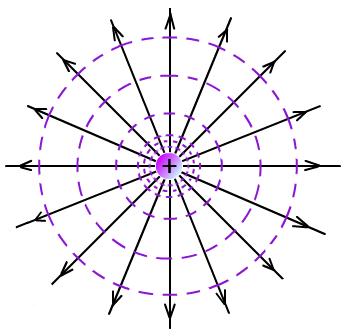
\includegraphics[width=5cm]{equipotential.png}
	\caption{Schematic of a point charge. The solid black lines are the electric field lines. The
		purple dashed lines are the equipotential lines.}
	\label{fig::equipotential}
\end{figure}

\section*{Procedure}
In today's lab, you will use the electric field mapping board to map lines of equipotential, which you will then use to draw the electric field.

n this lab, we'll be mapping out the equipotential lines for several configurations.
\begin{enumerate}
	\item{Choose a configuration board (see Figure~\ref{fig:config_board}). This board may be in the front or back of the classroom.}
	\item{Copy the schematic onto a separate sheet of paper. Your instructor should teach you how to do this accurately.}
	\item{Turn the mapping board over (see Figure~\ref{fig:mapping_board}). Screw the configuration board into the bottom of the mapping board.}
	\item{Turn the mapping board right-side-up.}
	\item{Using either tape or the legs of the mapping board, fix the schematic onto the top of the mapping board.}
	\item{In your notes, sketch a prediction of what both the electric field lines and equipotential lines will look like.}
	\item{Use the probe to measure the voltage on the mapping board. Your instructor should teach you how to operate the multimeter and the probe if you do not know how.}
	\item{Select a voltage (around 3 V is a good start). Mark the spot where you measured the voltage with a pencil, like in Figure~\ref{fig:pencil}. Keep probing for this voltage and marking the spot until you have enough points to form a curve (at least five points).\label{itm:voltselect_loop_start}}
	\item{Once you have at least five points on your equipotential curve, connect the points. Remember to write down what voltage you measured next to the curve.\label{itm:voltselect_loop_end}}
	\item{Repeat steps~\ref{itm:voltselect_loop_start}--\ref{itm:voltselect_loop_end} until you have at least five different equipotential curves.}
	\item{Repeat the entire process for one additional configuration.}
\end{enumerate}

\begin{figure}[hbt!]
	\begin{center}
		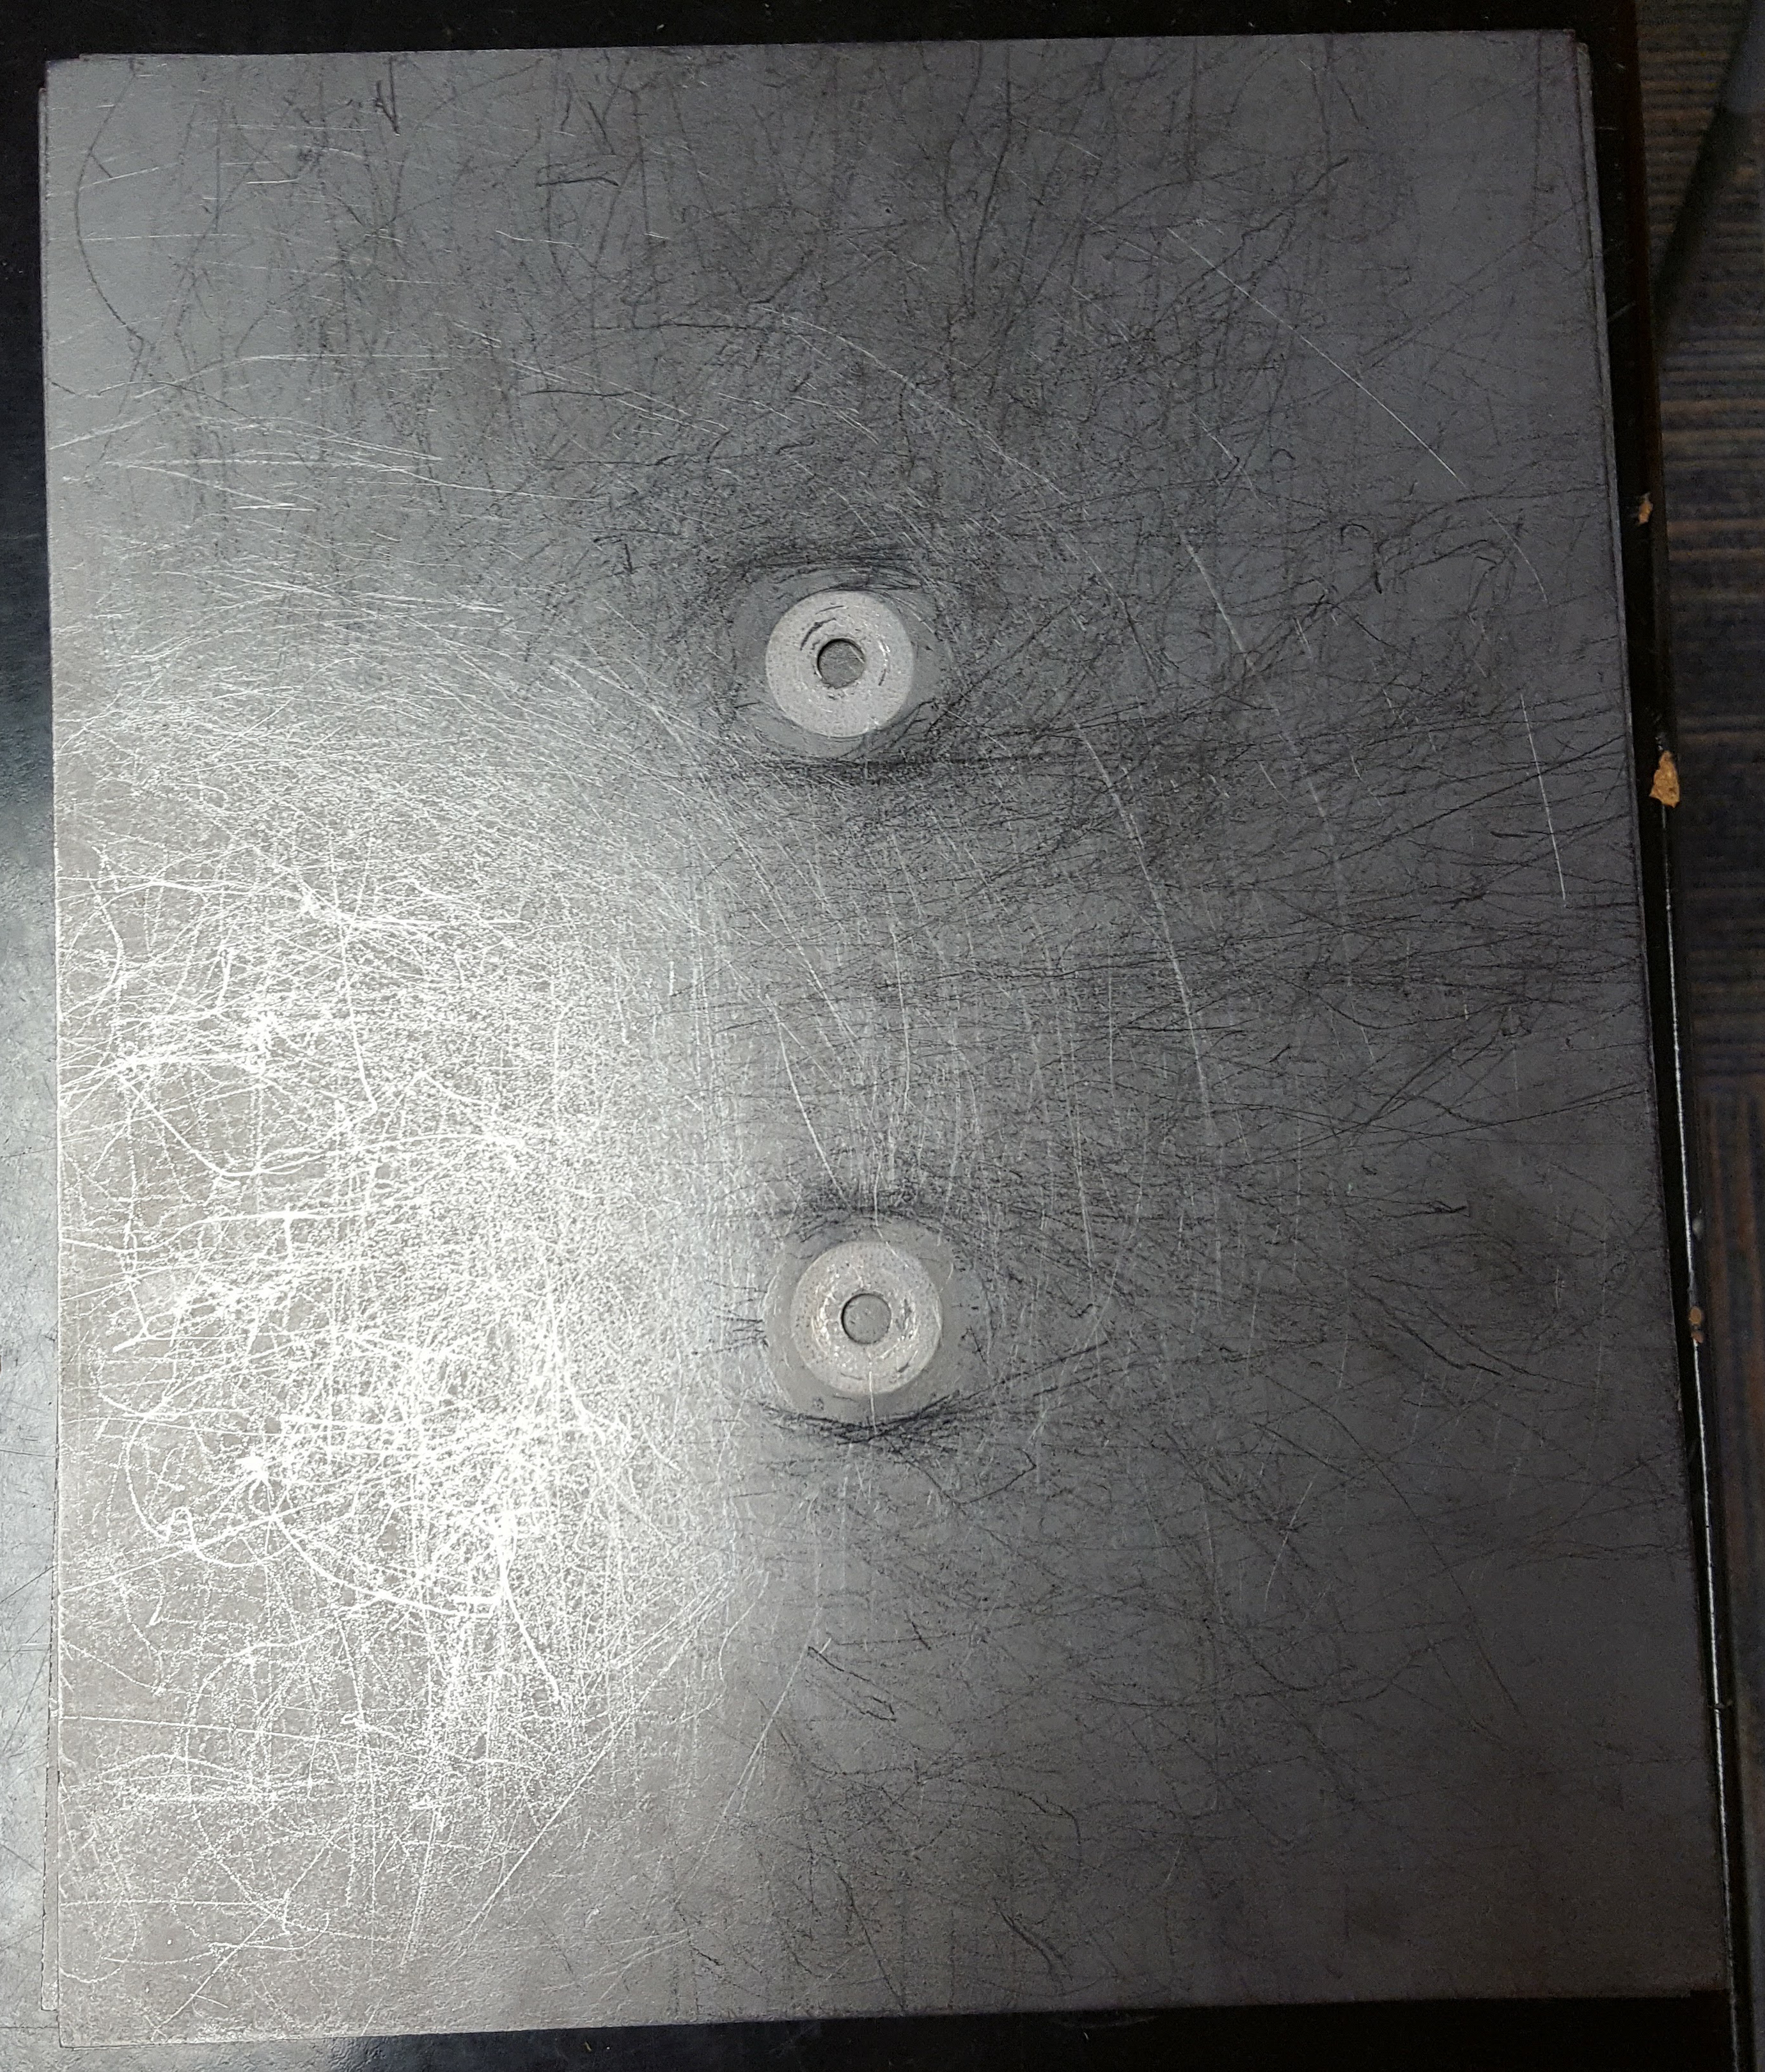
\includegraphics[width=0.5\textwidth]{config_board}
		\caption{An example of a configuration board.}
		\label{fig:config_board}
	\end{center}
\end{figure}

\begin{figure}[hbt!]
	\begin{center}
		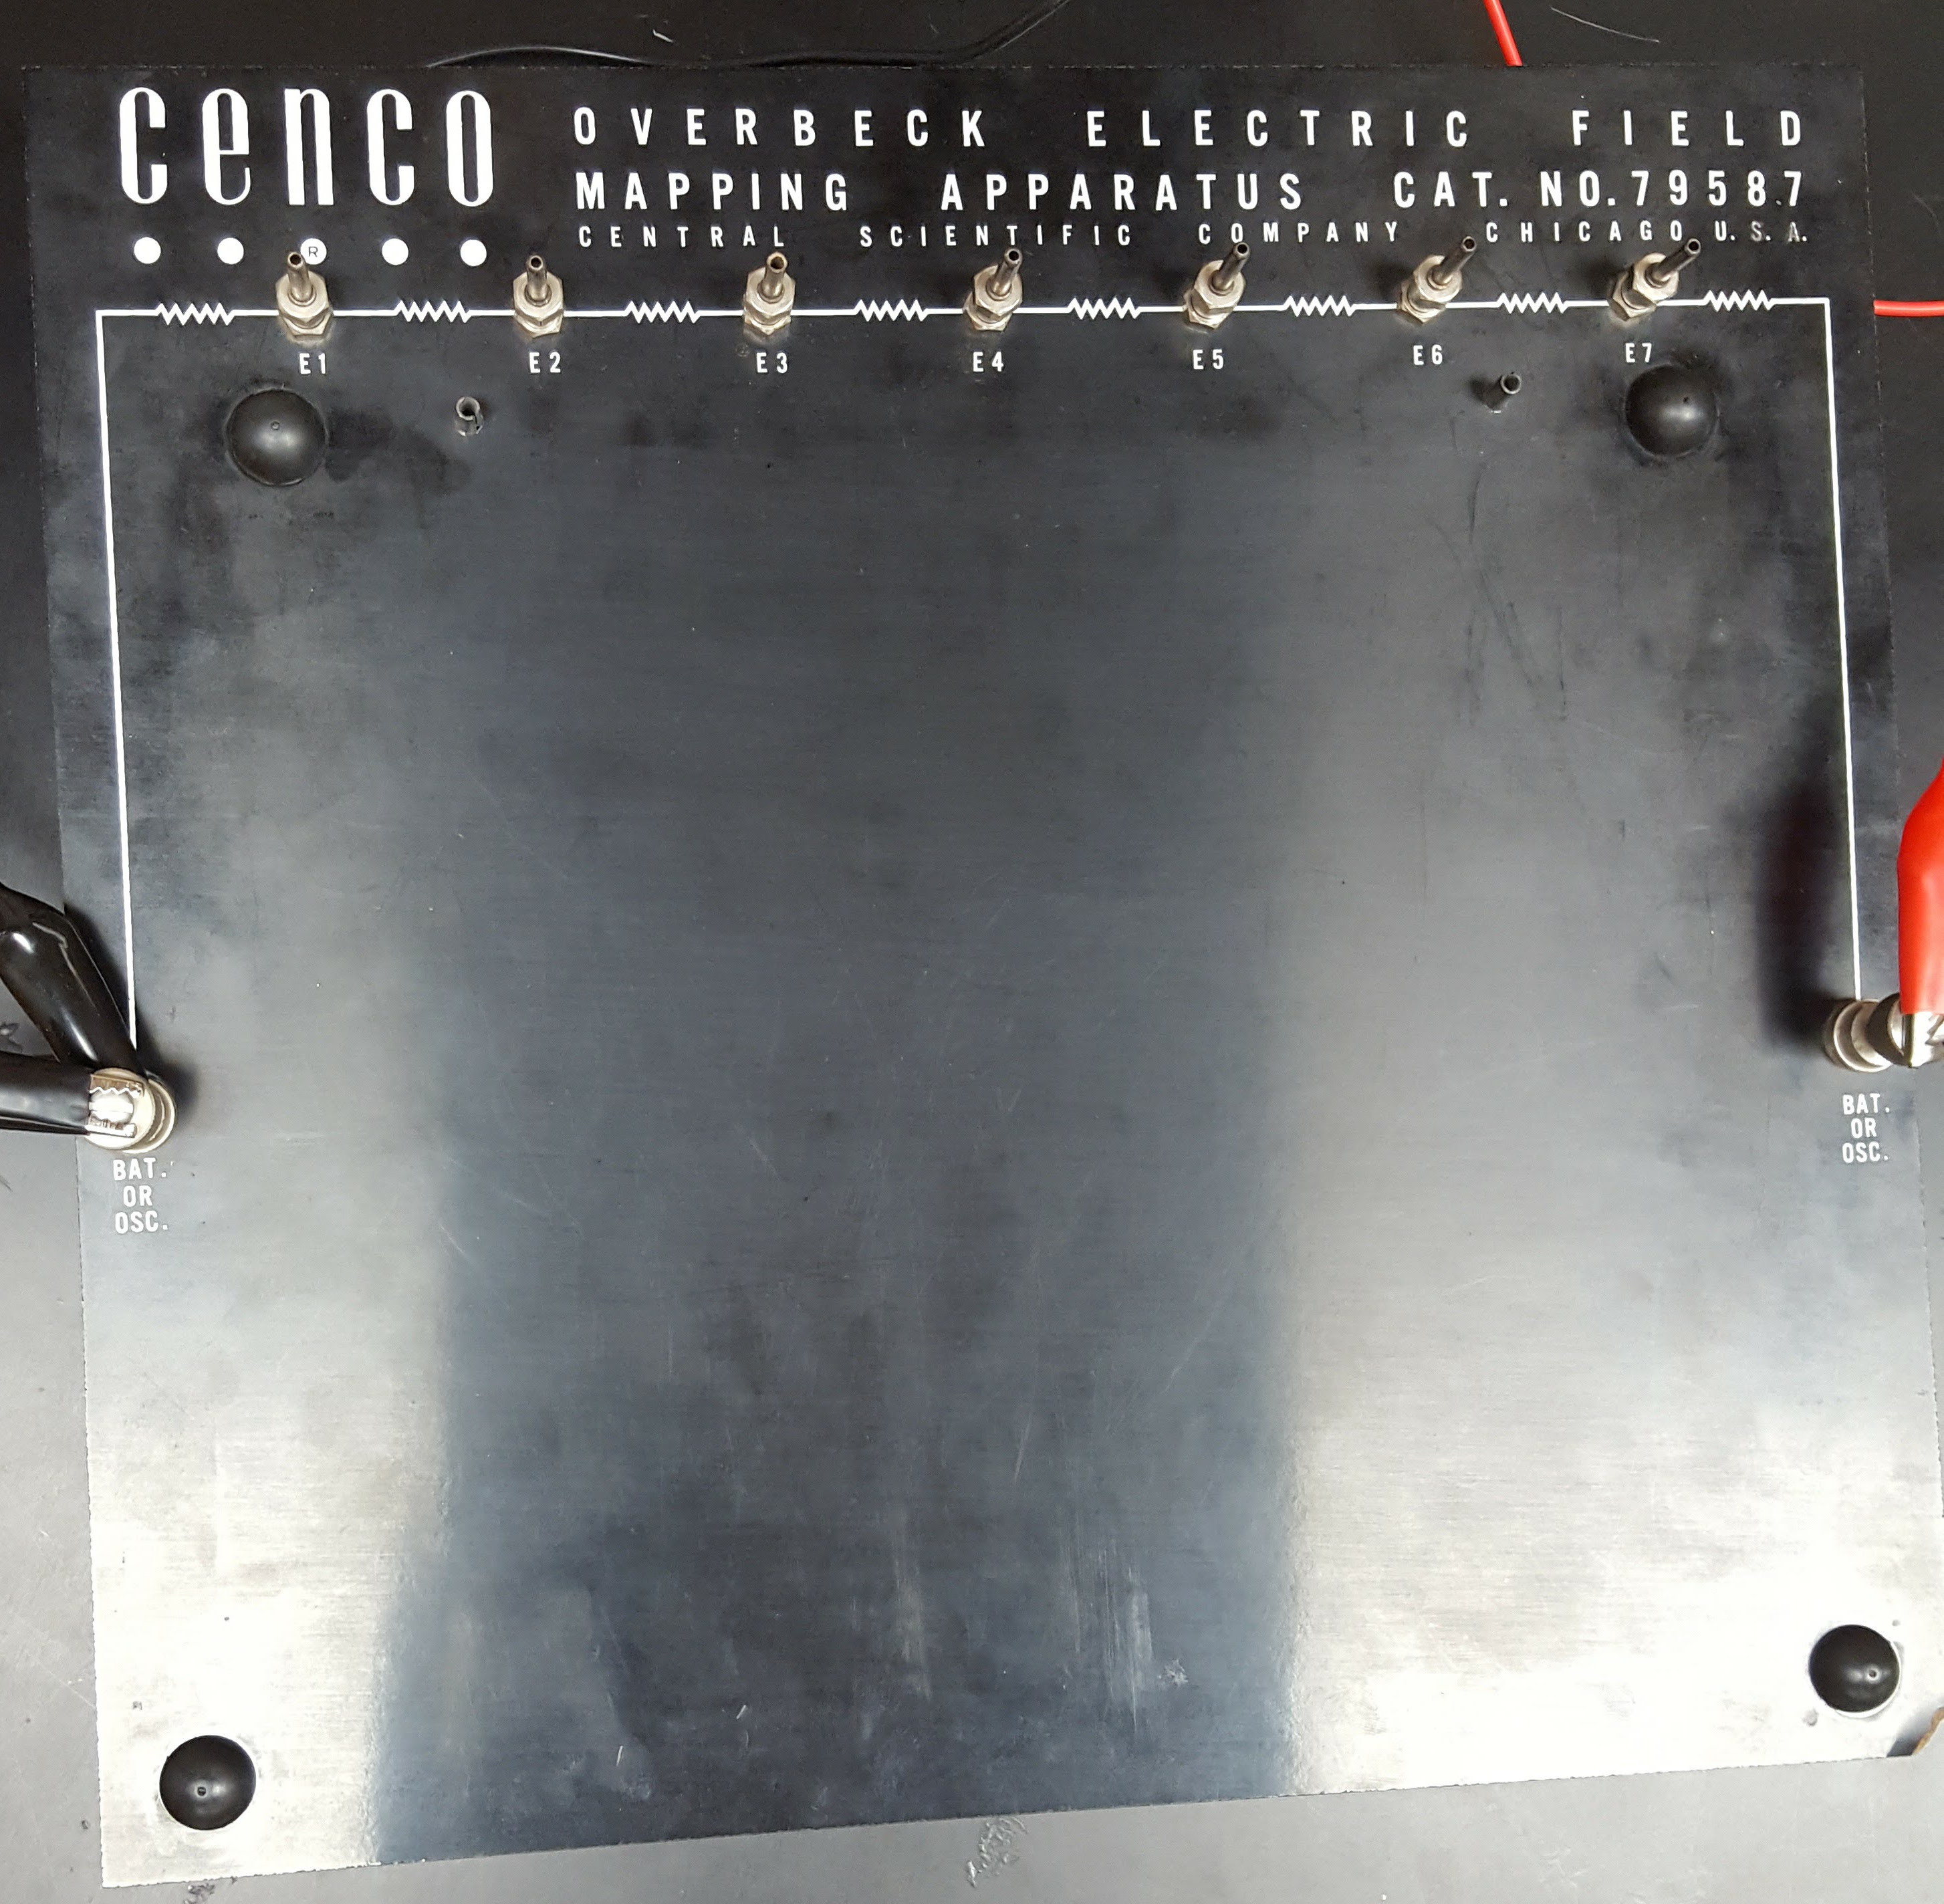
\includegraphics[width=0.5\textwidth]{mapping_board}
		\caption{The a mapping board.}
		\label{fig:mapping_board}
	\end{center}
\end{figure}

\begin{figure}[htb!]
	\begin{center}
		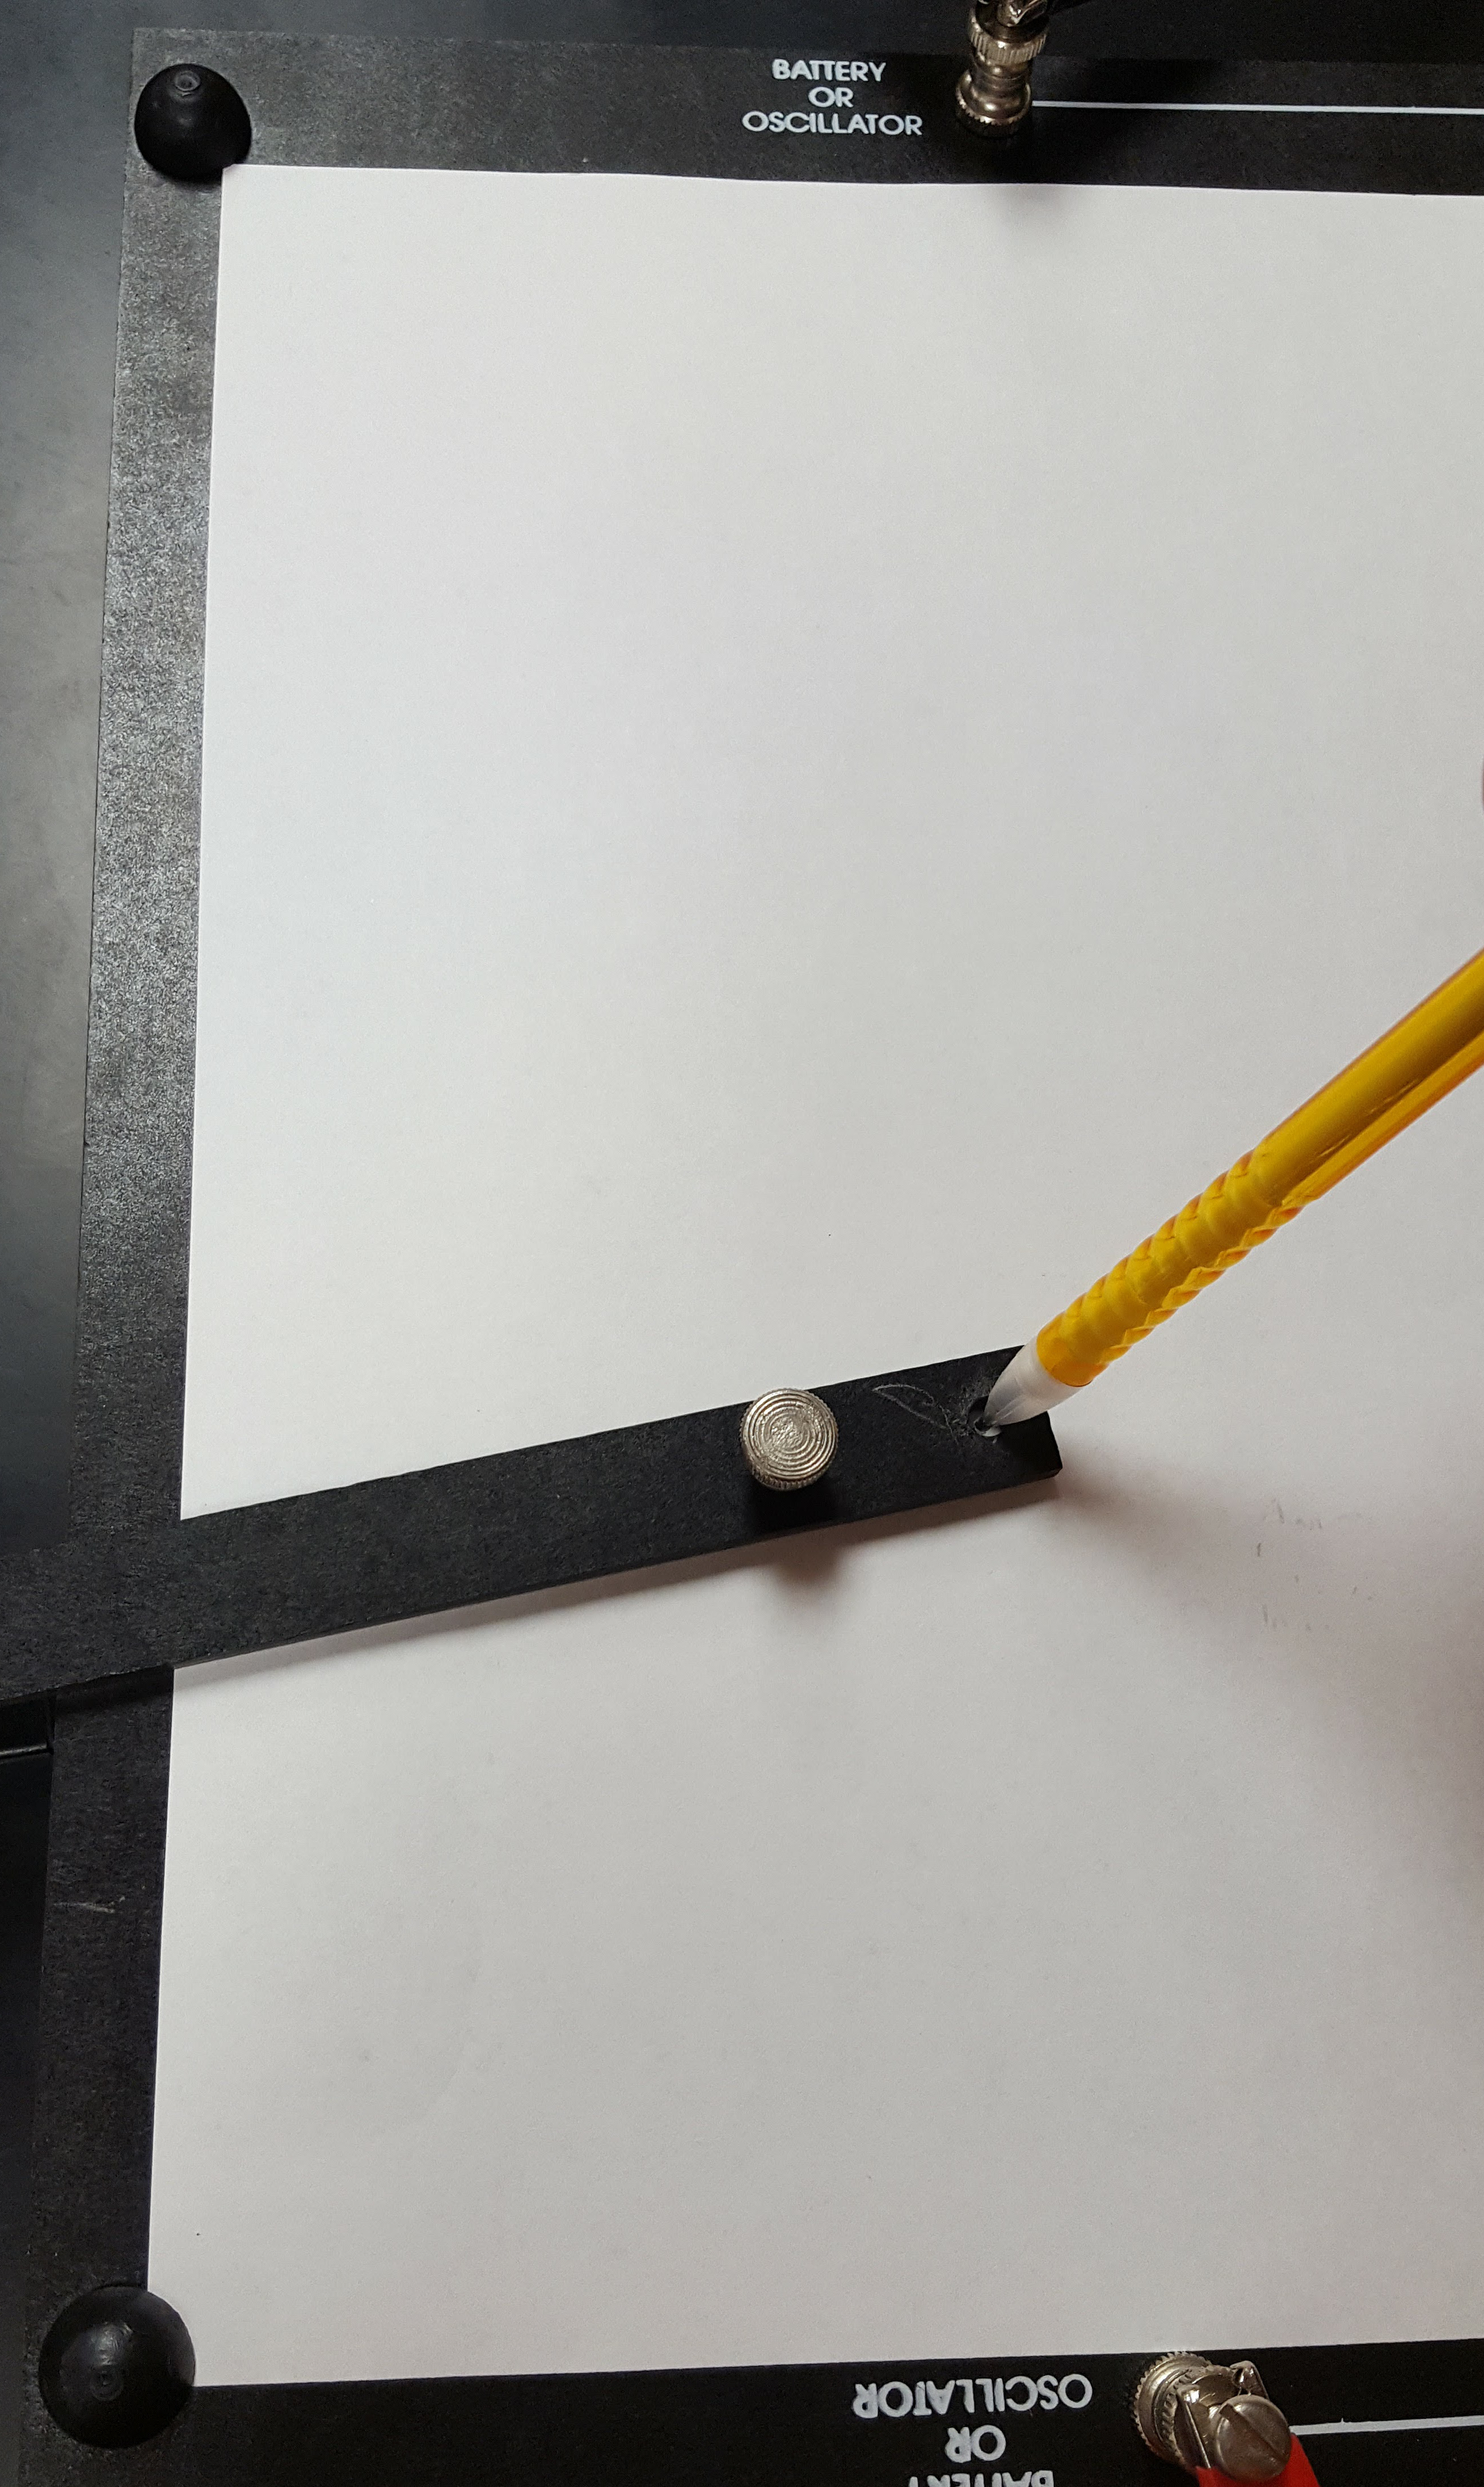
\includegraphics[width=0.25\textwidth]{pencil}
		\caption{How to mark on the paper with a pencil. Note that the pencil is in the hole.}
		\label{fig:pencil}
	\end{center}
\end{figure}



\section*{Analysis Questions}
\begin{enumerate}
	\item Explain any discrepancies between your predicted and measured results equipotential/field lines.
	\item For each configuration, pick three points and approximate the magnitude of the electric field at that point (\textit{Hint: measure the distance between two nearby equipotential curves, then you have $\Delta r$ and $\Delta V$, so you can find $\vec{E}$})
	\item Explain why equipotential lines and electric field lines must be perpendicular.
	\item Is it ever possible for two different equipotential lines to cross one another?
\end{enumerate}

\end{document}